\section{Limitations of Orchestration Decidability}
\label{chap:orchestration:decidability}

\mnote{Achieving optimality}
We have introduced the orchestration problem as the problem to find a consistent orchestration if it exists.
This is equivalent to the existence of an optimal orchestration function.
We can distinguish two approaches to ensure that the orchestration function is optimal.
Let $P$ be the problem space, i.e., all possible orchestrations of given transformations, and let $S_{i}$ be the solution space with those orders that yield consistent models for a specific input $i$ of models and changes to them.
\begin{properdescription}
    \item[Strategy Definition:] Define a strategy that explores the problem space $P$ to find one of the sequences in the solution space $S_{i}$ if $S_{i} \neq \emptyset$.
    \item[Transformation Restriction:] Define a \emph{well-behavedness} property for transformations that ensures that executing the transformations in any order often enough they yield consistent models if $S_{i} \neq \emptyset$. This means, for any given input $i$ there is an $n \in \mathbb{N}$ such that $\forall s \in P : \abs{s} > n \Rightarrow s \in S_{i}$.
\end{properdescription}

\mnote{Restrictions to transformations}
In the latter case, the orchestration function only needs to return orders that are longer than a specific length to be optimal.
This means, performing an iterative execution of the transformations leads to a consistent result.
Since optimality is a property of an orchestration function with respect to a set of transformations, defining a \emph{well-behavedness} property for transformations to ease finding an optimal orchestration function will potentially not concern a single transformation but the set of them.
This can easily contradict our assumption of independent development and reuse, or lead to restrictions of transformations that are not practical anymore.

\mnote{Section summary}
In the following, we first investigate the possibility to find an optimal orchestration function without restricting the transformations.
We define a general algorithm that realizes an application function, as in practice the function will be realized in terms of an algorithm that dynamically selects the next transformation to execute.
We then discuss its correctness and termination and relate it to the orchestration problem.
After proving undecidability of the orchestration problem, we discuss the possibilities to restrict transformations such that the problem becomes decidable.
Finally, we shortly discuss confluence as a considerable property of transformation networks.


\subsection{An Algorithm for Application Functions}
\label{chap:orchestration:decidability:algorithm}

\newcommand{\applyalgexecuted}{\sequence{\transformation{t}_{\mathvariable{executed}}}}
\newcommand{\applyalggenerated}{\sequence{\changetuple{\metamodeltuple{M}, \mathvariable{generated}}}}
\begin{algorithm}
    \begin{algorithmic}[1]
    \Procedure{$\function{Apply}$}{$\transformationset{T}, 
    \modeltuple{m} %= \tupled{\model{m}{1}, \dots, \model{m}{n}}
    , \changetuple{\metamodeltuple{M}} %= \tupled{\change{\metamodel{M}{1}}, \dots, \change{\metamodel{M}{n}}}
    $}
        \State $\mathvariable{isConsistent}$ $\leftarrow$ $\function{CheckConsistency}(\transformationset{T}, \modeltuple{m})$
        \If{$\neg \mathvariable{isConsistent}$}
            \State \Return{$\bot$}
        \EndIf
        \State $\applyalgexecuted \leftarrow \sequenced{}$
        \State $\applyalggenerated \leftarrow \sequenced{}$
        \State $\transformation{t}_\mathvariable{next}$ $\leftarrow$ $\function{Orchestrate}_{\transformationset{T}}(\modeltuple{m}, \changetuple{\metamodeltuple{M}}, \applyalgexecuted, \applyalggenerated)$ \label{algo:orchestration:application:line:startorchestrate}
        \While{$\transformation{t}_\mathvariable{next} \neq \bot$}
            \State $(\modeltuple{m}, \changetuple{\metamodeltuple{M}})$ $\leftarrow$ $\generalizationfunction{\metamodeltuple{M}, \transformation{t}_\mathvariable{next}}(\modeltuple{m}, \changetuple{\metamodeltuple{M}})$ \label{algo:orchestration:application:line:stepcalculation}
            \State $\applyalgexecuted \gets \applyalgexecuted + \transformation{t}_\mathvariable{next}$
            \State $\applyalggenerated \gets \applyalggenerated + \changetuple{\metamodeltuple{M}}$
            \State $\transformation{t}_\mathvariable{next}$ $\leftarrow$ $\function{Orchestrate}_{\transformationset{T}}(\modeltuple{m}, \changetuple{\metamodeltuple{M}}, \applyalgexecuted, \applyalggenerated)$
        \EndWhile \label{algo:orchestration:application:line:endorchestrate}
        %\State $\tupled{\model{m}{1}, \dots, \model{m}{n}} \leftarrow \modeltuple{m}$
        %\State $\tupled{\change{\metamodel{M}{1}}, \dots, \change{\metamodel{M}{n}}} \leftarrow \changetuple{\metamodeltuple{M}}$
        \State $\modeltuple{m}_\mathvariable{res} \leftarrow \changetuple{\metamodeltuple{M}}(\metamodeltuple{m})$ %\tupled{\change{\metamodel{M}{1}}(\model{m}{1}), \dots, \change{\metamodel{M}{n}}(\model{m}{n})}$
        \State $\mathvariable{isConsistent}$ $\leftarrow$ $\function{CheckConsistency}(\transformationset{T}, \modeltuple{m}_\mathvariable{res})$ \label{algo:orchestration:application:line:startconsistencycheck}
        \If{$\neg \mathvariable{isConsistent}$}
            \State \Return{$\bot$}
        \EndIf \label{algo:orchestration:application:line:endconsistencycheck}
        % \For{$\transformation{t} \in \transformationset{T}$} \label{algo:orchestration:application:line:startcheckconsistency}
        %     %\State $(\consistencyrelation{CR}{}, \consistencypreservationrule{\consistencyrelation{CR}{}}) \leftarrow \transformation{t}$
        %     \State $\mathvariable{isConsistent}$ $\leftarrow$ $\function{CheckConsistency}_{\metamodeltuple{M}}(\modeltuple{m}_{res}, \transformation{t}$) %\consistencyrelation{CR}{})$
        %     \If{$\neq \mathvariable{isConsistent}$}
        %         \State \Return{$\bot$}
        %     \EndIf
        % \EndFor \label{algo:orchestration:application:line:endcheckconsistency}
        \State \Return{$\modeltuple{m}_\mathvariable{res}$} \label{algo:orchestration:application:line:returnresult}
    \EndProcedure
\end{algorithmic}
    \caption[Application function implementation]{Application function implementation.}
    \label{algo:orchestration:application}
\end{algorithm}

\mnote{Algorithm for application function}
We have so far discussed the orchestration and application functions as mathematical functions.
In practice, they will be implemented as algorithms.
In \autoref{algo:orchestration:application}, we propose an algorithm that realizes an application function.
It also encodes the orchestration function, because an algorithm for the orchestration function will not determine a complete sequence of transformations for given models and changes but dynamically select the transformation to be executed next.
As soon as the orchestration function determines no further transformation for execution, the algorithm returns the resulting models if they are consistent and $\bot$ otherwise.

\mnote{Independent from actual transformations}
An application function according to \autoref{def:applicationfunction} is parametrized by an orchestration function, which, in turn, is parametrized by the set of transformations $\transformationset{T}$ that it is supposed to be executed on.
A transformation network according to \autoref{def:transformationnetwork} is defined to consist of a set of transformations and an application function, which may suggest that both the application as well as the orchestration function can be defined specific for one network.
\autoref{algo:orchestration:application} reflects this by assuming an \function{Orchestrate} function that is specific for a set of transformations.
It may, however, be implemented by a generic function that works independent from the actual transformations and, instead, accepts them as a parameter.
We do, however, focus on a general algorithm and an \function{Orchestrate} function that can be applied to any set of transformations.
In that case, the algorithm does not realize a single application function but actually a family of application functions for all possible transformation sets $\transformationset{T}$.

\mnote{Dynamic selection of next transformation}
The dynamic selection of transformations is realized by an \function{Orchestrate} function and stops as soon as no further transformations to apply are delivered.
The latter may be the case because the models are already consistent or because no further transformations can be applied.
It is essential that \function{Orchestrate} only returns a transformation that can be applied to the models and current changes, because otherwise its application by the $\generalizationfunction{}$ function in \autoref{algo:orchestration:application:line:stepcalculation} would fail.
The complete logic of the orchestration function is combined with the application of the delivered sequence in Lines~\ref{algo:orchestration:application:line:startorchestrate}--\ref{algo:orchestration:application:line:endorchestrate}.
Since, in practice, the selection of transformations has to be performed dynamically anyway, an implementation of the orchestration function always needs to apply the transformations.
Thus, a separation of the orchestration function into a separate algorithm, which performs the same steps as in Lines~\ref{algo:orchestration:application:line:startorchestrate}--\ref{algo:orchestration:application:line:endorchestrate}, leads to a redundancy by applying the transformations both in the separate orchestration algorithm as well as in the application algorithm.

\mnote{History of changes and transformations}
The \function{Orchestrate} function receives the history of executed transformations and generated changes, because if the complete orchestration function was implemented in a separate method, it would also be able to use that information to determine a proper orchestration.
Otherwise, its expressiveness would be restricted with respect to the definition of an orchestration function, because that function makes a global decision for all transformations to execute based on the original input, which is not available to the \function{Orchestrate} function after its first execution anymore.
In a practical implementation of that function, the history may not be considered or truncated, depending on the information necessary for the implemented orchestration strategy.

\mnote{Strategies for selecting next transformation}
The \function{Orchestrate} function may implement different strategies for selecting the next transformation, which we later discuss in more detail.
One simple strategy would execute the same order of transformations iteratively, thus always executing the transformation that was not executed for the longest time.
Another reasonable strategy would be to manage a queue of transformations.
After executing one transformation, all transformations that are adjacent to the metamodels of the two models that were modified by the transformation are enqueued if they were not enqueued yet.
This ensures that those transformations that can process changes that have just been produced by another transformation are executed next.
Both these strategies are independent from the actual transformations and could thus be implemented in a function that can be used for any set of transformations $\transformationset{T}$.
In \autoref{chap:orchestration:algorithm}, we discuss a specific orchestration strategy.
Until then, the actual strategy is not important and any of the exemplified ones can be imagined.

\mnote{Assumed additional functions}
Next to \function{Orchestrate}, the algorithm uses the external functions $\generalizationfunction{}$ and \function{CheckConsistency}.
The $\generalizationfunction{}$ function is the generalization function, which simply applies the given transformation to the appropriate models of the given tuple, as defined in \autoref{def:generalizationfunction}.
The \function{CheckConsistency} function checks whether the given models are consistent to the set of transformations, according to \autoref{def:consistencytransformation}.
This function can be implemented in two ways.
First, it may be implemented as an explicit check regarding the consistency relations of the transformations.
If the transformations are defined by their consistency relations, from which a transformations language derives the consistency preservation rules, such as \gls{QVTR}, the models can be checked regarding the given relations.
In case of \gls{QVTR}, the transformations can be executed in \emph{checkonly mode}~\cite[Sec.~7.9]{qvt}.
Second, it may be implemented by (virtually) executing the consistency preservation rules and checking whether their execution performs changes.
If the transformations are hippocratic according to \autoref{def:hippocratictransformation}, i.e., if they do not perform changes when the models are already consistent, consistency can be checked this way.
This is always necessary when the consistency relations are not explicitly given but are implicitly defined as the fixed points of the consistency preservation rules, such as for transformations defined in \gls{QVTO}.
Due to their simplicity, we do not provide an explicit implementation of these two functions.


\subsection{Correctness and Termination of the Algorithm}
\label{chap:orchestration:decidability:correctness_termination}

\mnote{Algorithm as correct application function}
\autoref{algo:orchestration:application} is constructed to implement an application function according to \autoref{def:applicationfunction}.
It is designed to be correct, i.e., to return models only when they are consistent.
We show that the algorithm fulfills these properties in the following theorem.

\begin{theorem}[Apply Algorithm Correctness]
    The \function{Apply} function in \autoref{algo:orchestration:application} fulfills the functional behavior of an application function as defined in \autoref{def:applicationfunction} and is correct according to \autoref{def:applicationfunctioncorrectness}.
\end{theorem}

\begin{proof}
    The \function{Apply} function fulfills the input and output requirements of an application function according to \autoref{def:applicationfunction}.
    It returns a model tuple only in \autoref{algo:orchestration:application:line:returnresult}, which is achieved by applying the changes that the sequence of transformations as delivered by the orchestration function yields, which is realized as a repeated call of the \function{Orchestrate} function in Lines~\ref{algo:orchestration:application:line:startorchestrate}--\ref{algo:orchestration:application:line:endorchestrate}.
    Thus, \function{Apply} fulfills the definition of an application function.

    Correctness of an application function according to \autoref{def:applicationfunctioncorrectness} requires the output models, if not returning $\bot$, to be consistent to the consistency relations of all transformations, as long as the input models were consistent.
    The algorithm returns models only in \autoref{algo:orchestration:application:line:returnresult} and otherwise returns $\bot$ before.
    The returned models are always consistent to the consistency relations of all transformations, because Lines~\ref{algo:orchestration:application:line:startconsistencycheck}--\ref{algo:orchestration:application:line:endconsistencycheck} ensure this.
\end{proof}

\mnote{No termination guarantee}
In addition to being correct, the algorithm needs to terminate for every input.
The only source of non-termination is the loop for orchestrating transformations, as there are no recursions and further loops.
According to the definition, an orchestration function is defined to return a finite sequence of transformations, which would also result in a finite number of executions of the loop for orchestrating transformations.
The implementation by a dynamic selection of the next transformation to execute can, however, lead to an infinite sequence of transformations.
The \function{Orchestrate} function receives the list of previously executed transformations, as otherwise it would never be able to identify that, for example, always the same transformation sequence is executed and leads to the same changes, which means that the algorithm performs an infinite alternation.
We do, however, need to ensure that the \function{Orchestrate} function returns $\bot$ after a finite number of calls.

\mnote{Termination guarantee options}
If we assumed that we can achieve optimality for the orchestration function, we would have the guarantee that if a consistent orchestration exists, the function will find it.
There is, however, no restriction to what the orchestration function may return when there is no consistent orchestration.
Thus, we have the following two options to ensure termination.
\begin{longenumerate}
    \item We enable the orchestration function to identify whether a consistent orchestration exists.
    \item We find an upper bound for the number of necessary transformation executions. Then, if a higher number of transformations was executed, we cannot expect the algorithm to find consistent models anymore and thus abort it.
\end{longenumerate}

\mnote{Termination by upper bound}
As the simplest solution, an upper bound would restrict the number of necessary transformation executions.
We do, however, prove in the following that there is no such upper bound.
Afterwards, we show that identifying whether a consistent orchestration exists is not possible either.
This leads to the insight that we cannot guarantee termination of the algorithm with an optimal orchestration function.


%\subsection{Upper Execution Bound}

\mnote{No general upper bound}
With the example in \autoref{fig:orchestration:necessity_multiple_executions}, in which values are incremented by one during each execution of one specific transformation until a fixed but arbitrary value $x$ is reached, we were able to show \autoref{lemma:minimal_executions}.
It states that there can be transformation networks in which a transformation needs to be executed at least $x-1$ times for a fixed but arbitrary $x$ until consistent models are found.
Thus, any consistent orchestration contains that transformation at least $x-1$ times.
While we have used that insight in \autoref{theorem:orchestration_single} to show that executing each transformation only once is, in general, insufficient, we can also use it to show the more general statement that there is no maximal length for the orchestration of transformation networks, independent from the network size.

\begin{theorem}[Shortest Consistent Orchestration Upper Bound]
    \label{theorem:orchestration_fixed}
    For every $t_\mathvariable{size} \geq 3$ and every $n \geq 0$, there is a set of transformations $\transformationset{T}$ with $\abs{\transformationset{T}} > t_\mathvariable{size}$ such that there are models $\modeltuple{m}$ and changes $\changetuple{\metamodeltuple{M}}$ to them for which each possible orchestration function $\orcfunction{\transformationset{T}}$ with whom $\appfunction{\orcfunction{\transformationset{T}}}(\modeltuple{m}, \changetuple{\metamodeltuple{M}})$ is consistent delivers a transformation sequence with $\abs{\orcfunction{\transformationset{T}}(\modeltuple{m}, \changetuple{\metamodeltuple{M}})} > n$.
\end{theorem}

\begin{proof}
    We know from \autoref{lemma:minimal_executions} that $\transformationset{T}_\mathvariable{inc}$ requires at least $x-1$ executions of $\transformation{t}_{12}$ for the inputs defined in \autoref{lemma:minimal_executions} and the fixed but arbitrary value $x$.
    Thus, with $x \geq n+2$, we know that at least $x-1 \geq n+1$ executions of $\transformation{t}_{12}$ are necessary.
    Let $\modeltuple{m}$ and $\changetuple{\metamodeltuple{M}}$ be the inputs defined in \autoref{lemma:minimal_executions}.
    Then, for every orchestration function $\orcfunction{\transformationset{T}_\mathvariable{inc}}$ that delivers a consistent orchestration for $\modeltuple{m}$ and $\changetuple{\metamodeltuple{M}}$, we know that $\abs{\orcfunction{\transformationset{T}_\mathvariable{inc}}(\modeltuple{m}, \changetuple{\metamodeltuple{M}})} \geq x-1 \geq n+1 > n$.
    Since adding arbitrary transformations whose consistency preservation rules implement the identity function to a set of transformations does not alter the results of the network, we can construct a network of arbitrary size $\geq 3$ with the same behavior out of $\transformationset{T}_\mathvariable{inc}$ by adding such transformations.
    This proves the theorem by example.
\end{proof}

\mnote{No upper bound for deciding orchestration existence}
In consequence, there is no fixed value and no value depending on the transformation network size that defines an upper bound for the necessary number of transformation executions to yield consistent models, i.e., there is no upper bound for the shortest consistent orchestration.
Thus, we cannot abort the execution of the \function{Apply} function after a fixed number of loop iterations without the possibility that consistent models would have been found if the execution had proceeded and thus not ensuring optimality.


\subsection{Undecidability of the Orchestration Problem}

\mnote{Undecidability of consistent orchestration existence}
To ensure termination of the \function{Apply} algorithm with an optimal orchestration function, we need to identify the case that no consistent orchestration exists, because that is the only situation in which otherwise an infinite number of transformation executions is possible.
Unfortunately, we can show that this orchestration existence problem is undecidable.
We reduce the halting problem for Turing machines to the orchestration problem.
Thus, solving the orchestration problem would solve the halting problem.
We have published a simplified version of this proof, based on a more concise formalism, in previous work~\owncite{gleitze2021orchestration-FASE}.

\begin{figure}
    \centering
    \newcommand{\distance}{2.5em}

\begin{tikzpicture}[
    state/.style={draw, fill=white, circle, minimum size=1.5em, inner sep=0em},
]

% PRINCIPLE 1
% Original
\node[state] (princ1_A) {$A$};
\draw[-latex] (princ1_A) to [out=230, in=310, looseness=6] node[below] {$a$} (princ1_A);
\draw[-latex] ([xshift=-1em]princ1_A.west) -- node[above] {$i$} (princ1_A.west);
\draw[-latex] (princ1_A.east) -- node[above] {$o$} ([xshift=1em]princ1_A.east);
% Changed
\node[state, right=2.5*\distance of princ1_A] (princ1_A1) {$A_1$};
\node[state, below=\distance of princ1_A1] (princ1_A2) {$A_2$};
\draw[-latex] (princ1_A1) to [bend right=15] node[left] (princ1_middle_transition) {$a$} (princ1_A2);
\draw[-latex] (princ1_A2) to [bend right=15] node[right] {$a$} (princ1_A1);
\draw[-latex] ([xshift=-1em]princ1_A1.west) -- node[above] {$i$} (princ1_A1.west);
\draw[-latex] (princ1_A1.east) -- node[above] {$o$} ([xshift=1em]princ1_A1.east);
\draw[-latex] (princ1_A2.east) -- node[below] {$o$} ([xshift=1em]princ1_A2.east);

% PRINCIPLE 2
% Original
\node[state, right=1.7*\distance of princ1_A1] (princ2_A) {$A$};
\node[state, below=\distance of princ2_A] (princ2_B) {$B$};
\draw[-latex] (princ2_A) to [bend right=15] node[left] {$a$} (princ2_B);
\draw[-latex] (princ2_B) to [bend right=15] node[right] {$b$} (princ2_A);
\draw[-latex] ([xshift=-1em]princ2_A.west) -- node[above] {$i_A$} (princ2_A.west);
\draw[-latex] ([xshift=-1em]princ2_B.west) -- node[below] {$i_B$} (princ2_B.west);
\draw[-latex] (princ2_A.east) -- node[above] {$o_A$} ([xshift=1em]princ2_A.east);
\draw[-latex] (princ2_B.east) -- node[below] {$o_B$} ([xshift=1em]princ2_B.east);
% Changed
\node[state, right=2.5*\distance of princ2_A] (princ2_A1) {$A_1$};
\node[state, right=\distance of princ2_A1] (princ2_A2) {$A_2$};
\node[state, below=\distance of princ2_A1] (princ2_B1) {$B_1$};
\node[state, below=\distance of princ2_A2] (princ2_B2) {$B_2$};
\draw[-latex] (princ2_A1) -- node[left] (princ2_middle_transition) {$a$} (princ2_B1);
\draw[-latex] (princ2_B1) -- node[above left] {$b$} (princ2_A2);
\draw[-latex] (princ2_A2) -- node[left] {$a$} (princ2_B2);
\draw[-latex] (princ2_B2) .. controls ([xshift=0.65*\distance,yshift=-1.4em]princ2_B1.south) and ([xshift=-6.5em,yshift=-1.4em]princ2_B1.south) .. node[pos=0.7, left] {$b$} (princ2_A1);
\draw[-latex] ([xshift=-1em]princ2_A1.west) -- node[above] {$i_A$} (princ2_A1.west);
\draw[-latex] ([xshift=-1em]princ2_B1.west) -- node[below] {$i_B$} (princ2_B1.west);
\draw[-latex] (princ2_A1.east) -- node[above] {$o_A$} ([xshift=1em]princ2_A1.east);
\draw[-latex] (princ2_A2.east) -- node[above] {$o_A$} ([xshift=1em]princ2_A2.east);
\draw[-latex] (princ2_B1.east) -- node[below] {$o_B$} ([xshift=1em]princ2_B1.east);
\draw[-latex] (princ2_B2.east) -- node[below] {$o_B$} ([xshift=1em]princ2_B2.east);

% LABELS
\node[above, align=center] at ([yshift=1.5em]$(princ1_A)!0.5!(princ1_A1)$) {\emph{Principle 1:} Cycle Length $1$};
\node[above, align=center] at ([yshift=1.5em]$(princ2_A)!0.5!(princ2_A2)$) {\emph{Principle 2:} Cycle Length $2$};

% SEPARATOR
\draw[lightgray] ([yshift=2em]$(princ1_A1.north)!0.5!(princ2_A.north)$) -- ($(princ1_A2.south)!0.5!(princ2_B.south)$);

\draw[-latex] ([xshift=-1.3*\distance]princ1_middle_transition.west) -- node[above] {replace} ([xshift=-0.4*\distance]princ1_middle_transition.west);
\draw[-latex] ([xshift=-1.6*\distance]princ2_middle_transition.west) -- node[above] {replace} ([xshift=-0.7*\distance]princ2_middle_transition.west);
\end{tikzpicture}
    %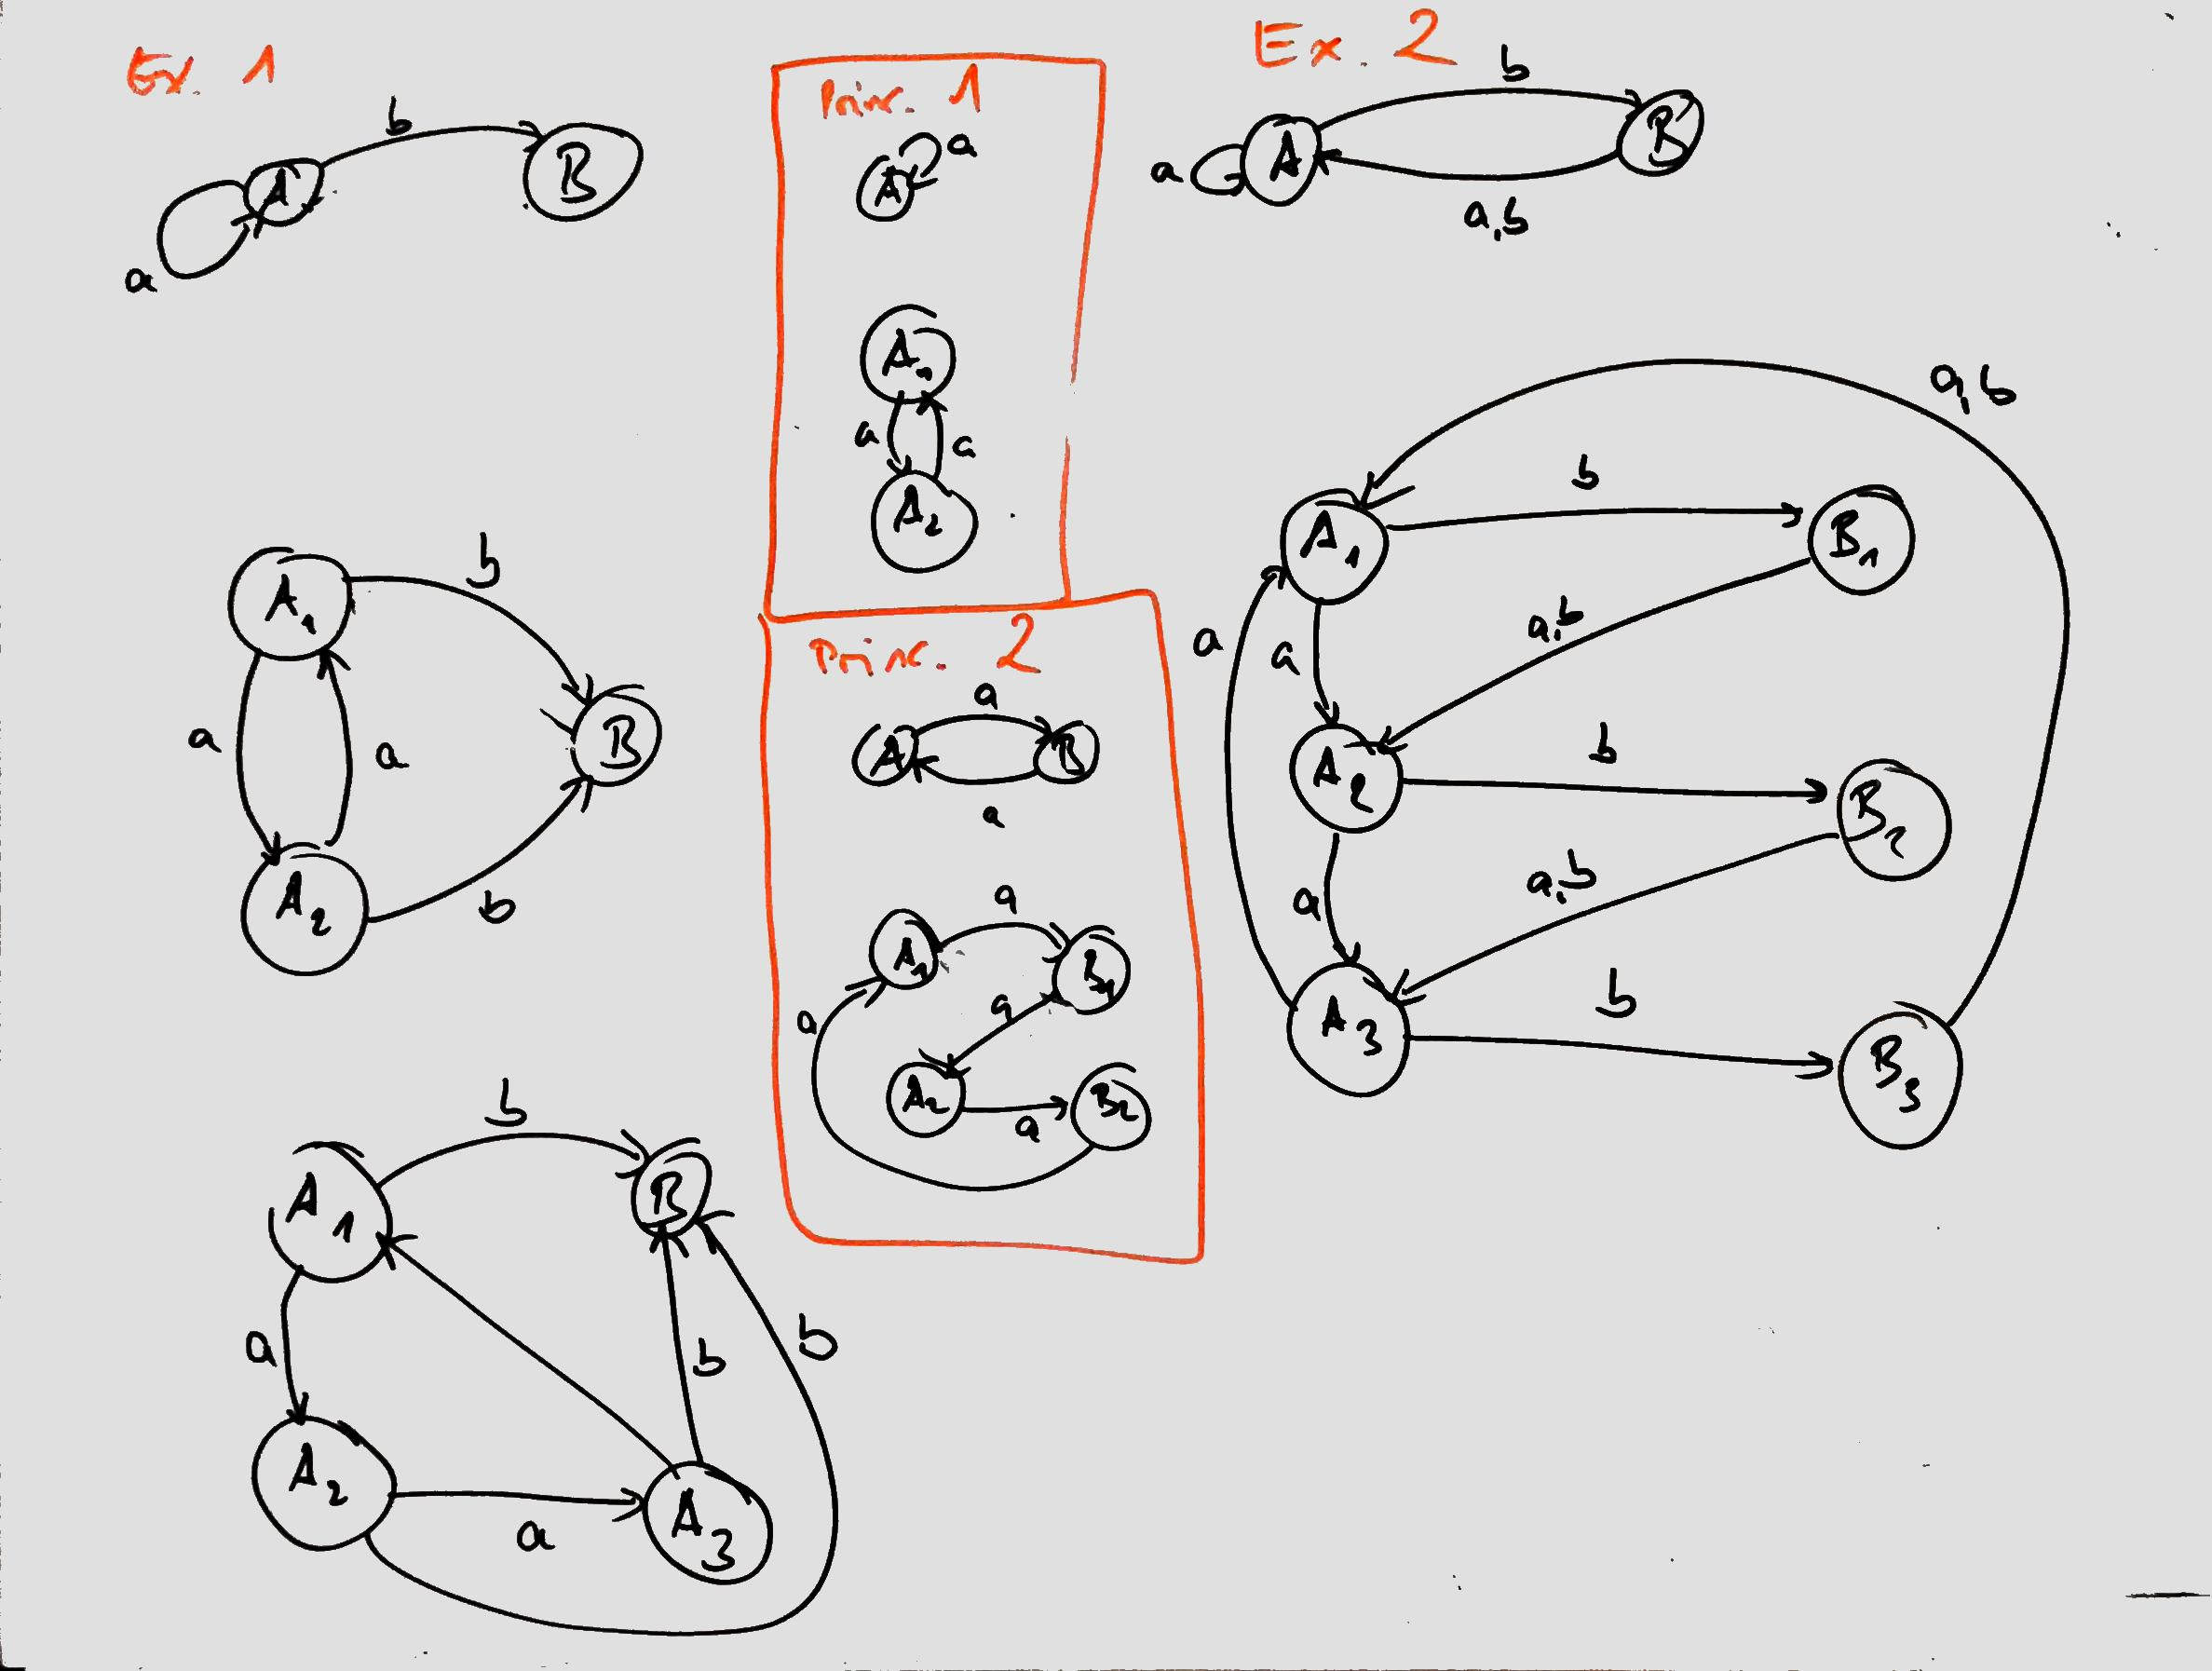
\includegraphics[width=0.45\textwidth]{figures/correctness/orchestration/cycle_elimination.jpg}\hfill
    %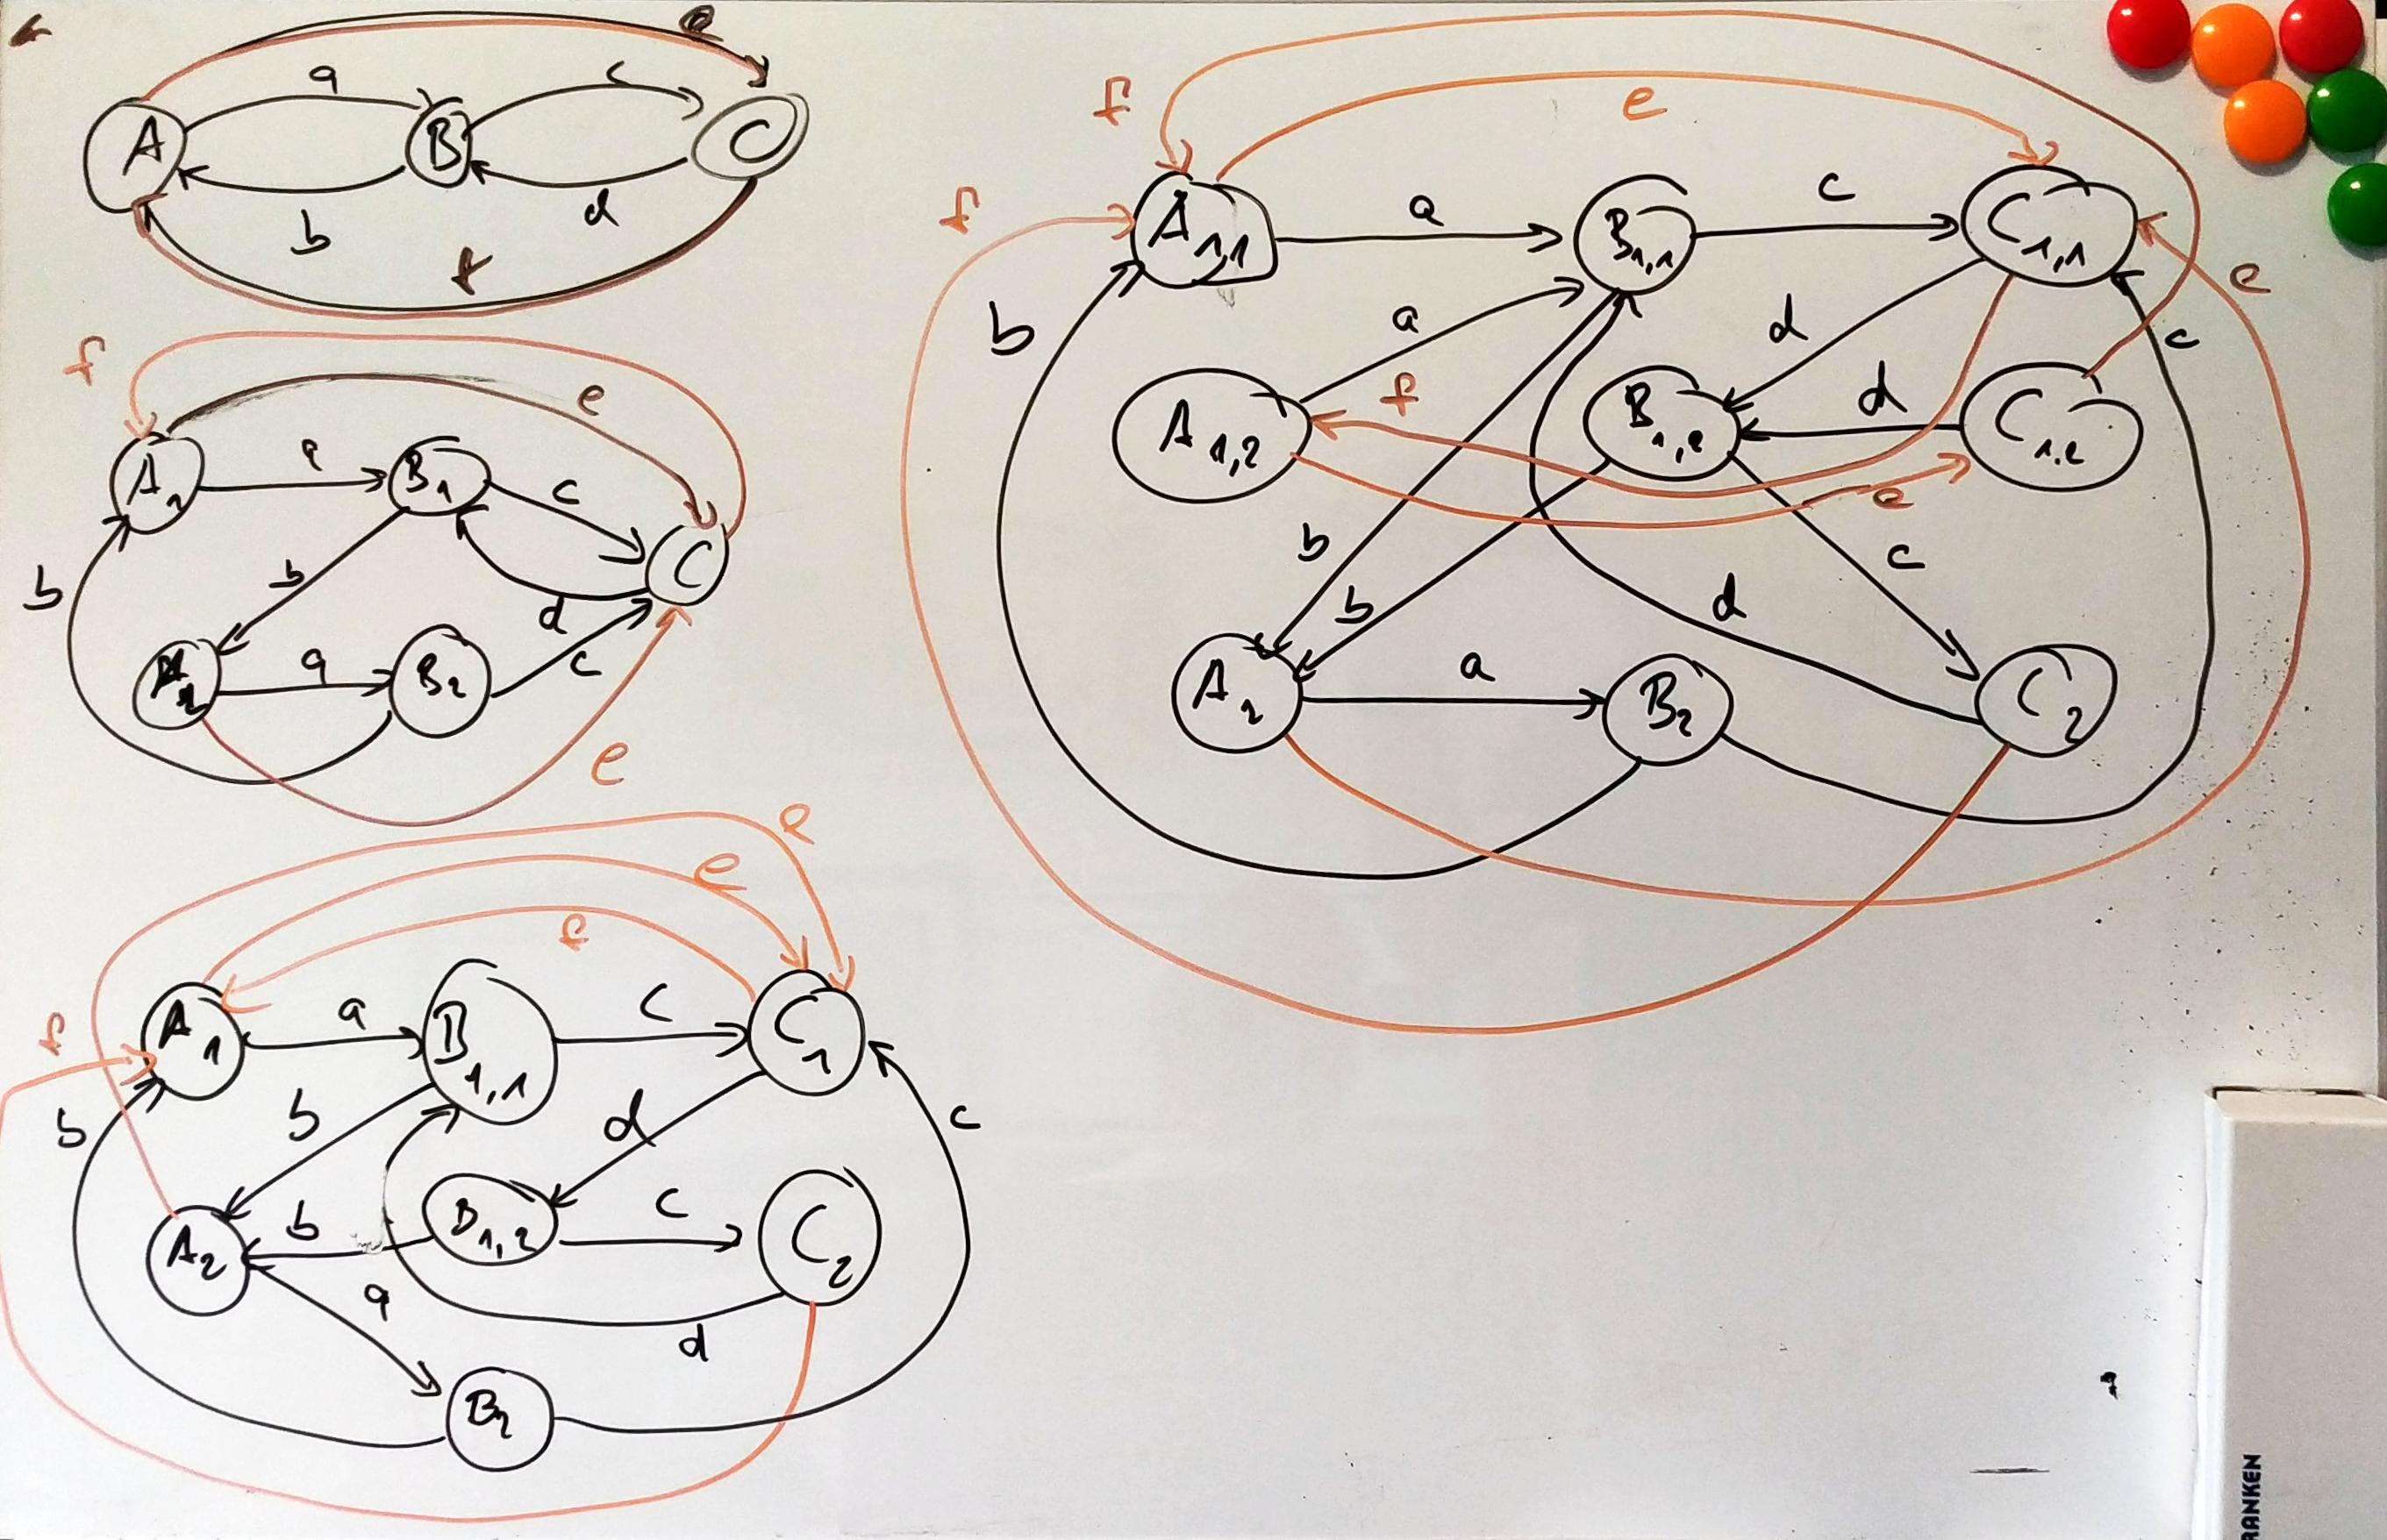
\includegraphics[width=0.54\textwidth]{figures/correctness/orchestration/cycle_elimination2.jpg}
    \caption[Cycle elimination in Turing machine transition functions]{Principles to eliminate cycles of length $\leq 2$ in the transition function of a Turing machine. $i$ and $o$ are placeholders for all incoming and outgoing transitions of a state.}
    \label{fig:orchestration:cycle_elimination}
\end{figure}

\mnote{Assumptions for Turing machine}
Given a Turing machine $\TuringMachine$ over some alphabet $\Sigma$, we construct metamodels $\metamodeltuple{M}_{\TuringMachine}$ and a transformation network with a set of transformations $\transformationset{T}_{\TuringMachine}$, as well as initial models $\modeltuple{m}_{\TuringMachine, x} \in \metamodeltupleinstanceset{M_{\TuringMachine}}$ and changes $\changetuple{\metamodeltuple{M},\TuringMachine,x}$, for them for which a consistent orchestration exists if, and only if, $\TuringMachine$ halts on input $x \in \Sigma^*$.
Without loss of generality, we assume that the graph of the transition function of $\TuringMachine$ contains no cycles of length $\leq 2$.
This means that it contains no self-loops, i.e., that the transition function always changes the state, and that there is no cycle between two states.
This is without loss of generality, because cycles of these two lengths can be eliminated by replicating states.
A self-loop can be eliminated by duplicating the state with a cycle of length $2$ between the duplicated states, replicating all outgoing transitions for both states, and letting all incoming transitions go to one of these two states.
Likewise, eliminating cycles of length $2$ can be achieved by duplicating both involved states and replacing the cycle of length $2$ by one of length $4$, replicating all outgoing transitions for all states, and letting all incoming transitions go to one of the two states of each replicated one.
Inductively applying these duplication principles can eliminate all cycles of length $\leq 2$.
The two principles are depicted in \autoref{fig:orchestration:cycle_elimination}.

\mnote{Models representing Turing machine states}
We construct models that consist of a timestamp, the tape content, and the tape position.
We encode this into a metamodel $\metamodel{M}{\TuringMachine}$, whose instances represent exactly these contents.
In a simplified notation, which considers a model as a tuple of these three elements rather than a set of elements, the instances of such a metamodel are given by $\metamodelinstanceset{M}{\TuringMachine} \equalsperdefinition \mathbb{N}_0 \times \Sigma^* \times \mathbb{N}_0$.
A model $\model{m}{} \equalsperdefinition \tupled{\mathvariable{time}, \mathvariable{cont}, \mathvariable{pos}} \in \metamodelinstanceset{M}{\TuringMachine}$ then represents a tuple of timestamp, tape content, and tape position.
To represent the states of the Turing machine, we consider one such metamodel for each state of the Turing machine, although they are all equal.
Thus, $\metamodeltuple{M}_\TuringMachine \equalsperdefinition \tupled{\metamodel{M}{1, \TuringMachine}, \dots, \metamodel{M}{n, \TuringMachine}}$ with $n = \abs{Q_\TuringMachine}$ if we assume $Q_\TuringMachine = \setted{q_1, \dots, q_n}$ to be the set of states of $\TuringMachine$.
We define the following function that returns the state of the Turing machine represented by a metamodel:
\begin{align*}
     \function{Q} : \metamodel{M}{i,\TuringMachine} & \mapsto q_i
\end{align*}
We consider a transformation between each pair of metamodels whose represented states in the Turing machine have a transition between them.
Finally, we consider models instantiating each of the metamodels to be kept consistent by an appropriate definition of these transformations representing the transitions of the Turing machine.

\mnote{Transformations representing Turing machine transitions}
The transformations increment the timestamp, change the tape content, and update the tape position according to the transitions of $\TuringMachine$ if, and only if, the timestamp of one model is higher than the one of the other.
More formally, let $\Tr(q_1,q_2) \subseteq \Sigma \times \setted{-1,0,1} \times \Sigma$ be the transitions defined between the states $q_1 \in Q_\TuringMachine$ and $q_2 \in Q_\TuringMachine$, with $-1$, $0$, and~$1$ indicating the head movements \enquote{left}, \enquote{stay}, and \enquote{right}, respectively. 
We define a consistency preservation rule for the transformation between the metamodels $\metamodel{M}{i, \TuringMachine}$ and $\metamodel{M}{k, \TuringMachine}$, which realizes the transition between the represented states of the Turing machine, as follows.
\begin{align*}
    &
    \consistencypreservationrule{i,k}(\model{m}{i}, \model{m}{k}, \change{\metamodel{M}{i,\TuringMachine}}, \change{\metamodel{M}{k,\TuringMachine}}) \equalsperdefinition (\change{\metamodel{M}{i,\TuringMachine}}', \change{\metamodel{M}{k,\TuringMachine}}') 
    \quad \mathtextspacearound{with:} \\
    &
    \model{m}{i}' \equalsperdefinition \tupled{\mathvariable{time}_{\model{m}{i}'}, \sequence{\mathvariable{cont}_{\model{m}{i}'}}, \mathvariable{pos}_{\model{m}{i}'}} \equalsperdefinition \changetuple{\metamodel{M}{i,\TuringMachine}}(\model{m}{i}) \\
    &
    \model{m}{k}' \equalsperdefinition \tupled{\mathvariable{time}_{\model{m}{k}'}, \sequence{\mathvariable{cont}_{\model{m}{k}'}}, \mathvariable{pos}_{\model{m}{k}'}} \equalsperdefinition \changetuple{\metamodel{M}{k,\TuringMachine}}(\model{m}{k}) \\
    &
    \change{\metamodel{M}{i,\TuringMachine}}'(\model{m}{i}) \equalsperdefinition 
    \begin{cases}
        \tupled{\mathvariable{time}_{\model{m}{k}'} + 1, \mathvariable{cont}_{\model{m}{k}'}|_{\mathvariable{pos}_{\model{m}{k}'} \gets \mathvariable{repl}}, \mathvariable{pos}_{\model{m}{k}'} + \mathvariable{dir}}, \\
        \formulaskip[0.5em+0.05\difftoafiveimage]
            \ifmath \mathvariable{time}_{\model{m}{k}'} > \mathvariable{time}_{\model{m}{i}'} \; \land \\
        \formulaskip[0.8em+0.13\difftoafiveimage]
            \exists \tupled{\sequenceindex{\mathvariable{cont}_{\model{m}{k}'}}{\mathvariable{pos}_{\model{m}{k}'}}, \mathvariable{dir},\mathvariable{repl}} \in \Tr(Q(\metamodel{M}{k,\TuringMachine}),Q(\metamodel{M}{i,\TuringMachine}))\\[.4em]
        \model{m}{i}', \formulaskip 
        \otherwisemath
    \end{cases} \\
    &
    \change{\metamodel{M}{k,\TuringMachine}}'(\model{m}{k}) \equalsperdefinition 
    \begin{cases}
        \tupled{\mathvariable{time}_{\model{m}{i}'} + 1, \mathvariable{cont}_{\model{m}{i}'}|_{\mathvariable{pos}_{\model{m}{i}'} \gets \mathvariable{repl}}, \mathvariable{pos}_{\model{m}{i}'} + \mathvariable{dir}}, \\
        \formulaskip[0.5em+0.05\difftoafiveimage]
            \ifmath \mathvariable{time}_{\model{m}{i}'} > \mathvariable{time}_{\model{m}{k}'} \; \land \\
        \formulaskip[0.8em+0.13\difftoafiveimage]
            \exists \tupled{\sequenceindex{\mathvariable{cont}_{\model{m}{i}'}}{\mathvariable{pos}_{\model{m}{i}'}}, \mathvariable{dir},\mathvariable{repl}} \in \Tr(Q(\metamodel{M}{i,\TuringMachine}),Q(\metamodel{M}{k,\TuringMachine}))\\[.4em]
        \model{m}{k}', \formulaskip 
        \otherwisemath
    \end{cases}
\end{align*}
where $\mathvariable{cont}|_{\mathvariable{pos} \gets \mathvariable{repl}} \equalsperdefinition \sequenceindex{\mathvariable{cont}}{0 \dots \mathvariable{pos}-1} \cdot \mathvariable{repl} \cdot \sequenceindex{\mathvariable{cont}}{\mathvariable{pos}+1 \dots \abs{\mathvariable{cont}}-1}$.

\mnote{Implicit consistency relations}
The \modellevelconsistencyrelations are implicitly given by the fixed points of the consistency preservation rules.
For a consistency preservation rule $\consistencypreservationrule{i,k}$, we define:
\begin{align*}
    \consistencyrelation{CR}{i,k} \equalsperdefinition \setted{
    & 
    \tupled{\model{m}{i}, \model{m}{k}} \in \metamodelinstanceset{M}{i,\TuringMachine} \times \metamodelinstanceset{M}{k,\TuringMachine} \mid 
    \exists \model{m}{i}', \model{m}{k}', \change{\metamodel{M}{i,\TuringMachine}}, \change{\metamodel{M}{k,\TuringMachine}} : \\
    & 
    \consistencypreservationrule{i,k}(\model{m}{i}',\model{m}{k}',\change{\metamodel{M}{i,\TuringMachine}}, \change{\metamodel{M}{k,\TuringMachine}})(\model{m}{i}',\model{m}{k}') = \tupled{\model{m}{i}, \model{m}{k}}}
\end{align*} 
With this definition, each consistency preservation rule is correct, i.e., one application of it yields models that are consistent to its defined consistency relation.
This is because due to the assumption that the graph induced by the transition function of $\TuringMachine$ does not contain cycles of length $\leq 2$, there may be no cyclic transitions between the states which are represented by the models kept consistent by a single transformation.

\mnote{Transformations only for transitions}
We denote the set of all transformations realizing the transitions of $\TuringMachine$ as $\transformationset{T}_{\TuringMachine}$, containing transformations $\transformation{t}_{i,k} = \tupled{\consistencyrelation{CR}{i,k},\consistencypreservationrule{i,k}}$ for all metamodel pairs $\tupled{\metamodel{M}{i,\TuringMachine},\metamodel{M}{k,\TuringMachine}}$ for which a transition between the represented states in $Q_\TuringMachine$ exists, i.e., $\Tr(Q(\metamodel{M}{i,\TuringMachine}),Q(\metamodel{M}{k,\TuringMachine})) \neq \emptyset$.

\mnote{Representation of Turing machine start state}
Let $s \in Q_{\TuringMachine}$ be the initial state of $\TuringMachine$. We set
\parameterizeformat{
\begin{alignat*}{2}
    &
    \modeltuple{m}_{\TuringMachine, x} \equalsperdefinition \tupled{\model{m}{1,\TuringMachine,x}, \dots, \model{m}{n,\TuringMachine,x}} 
    #1 #2
    \withmath
    \model{m}{i, \TuringMachine, x} \equalsperdefinition \tupled{0, \varepsilon, 0} \\
    &
    \changetuple{\metamodeltuple{M},\TuringMachine,x} \equalsperdefinition \tupled{\change{\metamodel{M}{1},\TuringMachine,x}, \dots, \change{\metamodel{M}{n},\TuringMachine,x}}
    #1 #2
    \withmath 
    \change{\metamodel{M}{i},\TuringMachine,x}(\model{m}{i}) \equalsperdefinition 
    \begin{cases}
        \tupled{1,x,0}, & \ifmath Q(\metamodel{M}{i}) = s\\
        \model{m}{i}, & \otherwisemath
    \end{cases}
\end{alignat*}
}{\quad &&}{\\ & \formulaskip}%

\mnote{Reduction of halting problem to orchestration problem}
We can show that for every Turing machine, this construction of a transformation network out of it solves the halting problem if we are able to solve the orchestration problem.
First, we show an auxiliary lemma that proves that executing the transformations until all models are consistent terminates if, and only if, the according Turing machine halts.

\begin{lemma}[Halting to Orchestration Problem Reduction]
    \label{lemma:turing_machine_construction}
    Executing the transformations of $\transformationset{T}_{\TuringMachine}$ for the models $\modeltuple{m}_{\TuringMachine,x}$ and changes $\changetuple{\metamodeltuple{M},\TuringMachine,x}$ until all models are consistent terminates if, and only if, $\TuringMachine$ halts on input $x$.
	If executing the transformations terminates with the final changes $\changetuple{\metamodeltuple{M},f}$, then the model in $\modeltuple{m}_{f} \equalsperdefinition \changetuple{\metamodeltuple{M},f}(\modeltuple{m}_{\TuringMachine,x})$ with the highest timestamp contains $\TuringMachine(x)$ as tape content.
\end{lemma}

\begin{proof}
    Let $\changetuple{s}, s \in \mathbb{N}_0$ be the tuple of changes created after executing $s$ transformations and let $\modeltuple{m}_{s} = \tupled{\model{m}{1,s}, \dots, \model{m}{n,s}}\equalsperdefinition \changetuple{s}(\modeltuple{m}_{\TuringMachine,x})$ be the state of the models after applying that change.
    Then we can see the following per induction over the model states $\modeltuple{m}_{s}$:
	\begin{longenumerate}
        \item 
            There is at most one transformation $\transformation{t}_{i,k} \in \transformationset{T}_{\TuringMachine}$ such that $\tupled{\model{m}{i,s},\model{m}{k,s}}$ is not consistent to $\transformation{t}_{i,k}$, i.e., $\tupled{\model{m}{i,s},\model{m}{k,s}} \not\in \consistencyrelation{CR}{i,k}$.
            This follows from the definition of $\TuringMachine$ and the last executed transformation.
            Let us, in contrary, assume that there was a second transformation that could be executed, because the models are inconsistent. 
            We can distinguish whether the transformation involves any of $\model{m}{i,s},\model{m}{k,s}$ or not.
            If that transformation involves any of these two models, then $\TuringMachine$ would have been non-deterministic, because each transformation realizes a transition between the associated states of $\TuringMachine$.
            If that transformation involves none of these models, then one them must have been changed before, because otherwise they are consistent by construction of $\modeltuple{m}_{\TuringMachine,x}$.
            Let that changed model be $\model{m}{}'$.
            The transformation to which $\model{m}{}'$ and another model are inconsistent cannot be the one that was executed after $\model{m}{}'$ was changed, because its correctness ensures that the two are consistent afterwards.
            Again, due to $\TuringMachine$ being deterministic, there cannot be another transformation that needed to be executed after $\model{m}{}'$ was changed. 
            Thus, another model must have been changed later, which led to the inconsistency. Then, however, the transformation would have needed to be applied, because the other model was changed.
            Since another transformation was executed and, again, because of $\TuringMachine$ being deterministic, that inconsistency cannot occur, thus being a contradiction to the assumption.
        \item 
            There is exactly one model $(\mathvariable{time}_{h,s},\mathvariable{cont}_{h,s},\mathvariable{pos}_{h,s}) \equalsperdefinition \model{m}{h,s} \in \modeltuple{m}_{s}$ that has the highest timestamp $\mathvariable{time}_{h,s}$ of all models in $\modeltuple{m}_{s}$.
            This follows from the previous insight that there is always at most one transformation to which the models are not consistent and which can thus perform changes, and that this transformation involves the just changed model, which, per induction, has the highest timestamp of all models.
            Thus, this model must be $\model{m}{i,s}$ or $\model{m}{k,s}$.
            We assume without loss of generality $\model{m}{h,s} = \model{m}{i,s}$.            
		 \item
            If a $\transformation{t}_{i,k}$ exists to which $\tupled{\model{m}{i,s},\model{m}{k,s}}$ is not consistent, then $\model{m}{k,s+1}$ contains the same tape content and the same tape position as would result if $\TuringMachine$ was executed one step from the state encoded in $\model{m}{i,s}$ with tape content $\mathvariable{cont}_{i,s}$ and tape position $\mathvariable{pos}_{i,s}$.
		 	Additionally, $\model{m}{k,s+1}$ is the model with the highest timestamp of all models in $\modeltuple{m}_{s+1}$.
		 \item 
             $\modeltuple{m}_{s}$ is consistent to $\transformationset{T}_{\TuringMachine}$ and thus no further transformation can produce changes if, and only if, $\TuringMachine$ would halt in state $\model{m}{i,s}$ with tape content $\mathvariable{cont}_{i,s}$ and tape position $\mathvariable{pos}_{i,s}$.
             This is given by construction of the transformations, because a transformation can be executed if, and only if, the timestamp of the model is lower than the timestamp of a model to which a transformation is defined and if there is an according transition in $\Tr$ of $\TuringMachine$.
             Since the timestamp of $\model{m}{i,s}$ is higher than the timestamp of all other models, a transformation can be executed if, and only if, there is an according transition of $\TuringMachine$, thus the execution of transformations terminates exactly when $\TuringMachine$ halts.
		 	\qedhere
	\end{longenumerate}
\end{proof}

\mnote{Orchestration problem undecidability}
With this lemma, it is easy to see that we could decide the halting problem if we can decide whether a consistent orchestration for the transformation network constructed from a Turing machine exists.
In consequence, the orchestration problem is undecidable.

\begin{theorem}[Orchestration Problem Undecidability] \label{theorem:orchestration_problem_undecidability}
    The orchestration (existence) problem is undecidable.
\end{theorem}

\begin{proof}
    We have given the constructive proof for \autoref{lemma:turing_machine_construction} that any Turing machine can be simulated by a transformation network such that a repeated execution of transformations finds consistent models of which one contains the resulting tape content of the Turing machine if, and only if, the Turing machine halts.
    Thus, if we could decide the orchestration problem, we could decide whether a consistent orchestration exists. 
    The consistent orchestration for the given transformations is unique, as in each step there is always only one transformation that can be executed.
    In consequence, knowing that a consistent orchestration exists means, according to \autoref{lemma:turing_machine_construction}, that we can decide whether $\TuringMachine$ halts, i.e., we could decide the halting problem.
    Due to equivalence of the orchestration problem and the orchestration existence problem, according to \autoref{theorem:orchestrationproblemequivalence}, this also applies to the orchestration existence problem.
\end{proof}

\mnote{No optimal application functions}
According to \autoref{theorem:optimal_application_function_orchestration_problem}, we can only find an optimal application function if the orchestration problem is decidable.
Thus, we know that we cannot find such a function.

\begin{corollary}[Application Function Non-Optimality]
    \label{corollary:nooptimalapplication}
    Let $\appfunction{\orcfunction{\transformationset{T}}}$ be an application function. Then $\appfunction{\orcfunction{\transformationset{T}}}$ cannot be optimal.
\end{corollary}

\begin{proof}
    According to \autoref{theorem:optimal_application_function_orchestration_problem}, an optimal application function can only be defined if a solution for the orchestration problem exists.
    Due to \autoref{theorem:orchestration_problem_undecidability}, we know that the problem is undecidable and thus an optimal application function cannot be defined.
\end{proof}

\mnote{Algorithm cannot terminate and be optimal}
From this corollary, it also follows that we cannot implement the \function{Apply} function of the proposed algorithm in a way that it realizes an optimal application function and terminates for every possible input.

\begin{corollary}[Apply Algorithm Non-Optimality]
    \function{Apply} according to \autoref{algo:orchestration:application} cannot terminate and return consistent models whenever an orchestration exists that yields them exists for every possible input.
\end{corollary}

\begin{proof}
    If \function{Apply} always terminated and returned consistent models whenever there is an orchestration that yields them, it would implement an optimal application function. 
    According to \autoref{corollary:nooptimalapplication} an application function cannot be optimal.
\end{proof}

\mnote{Transformation restriction vs. conservativeness}
In consequence, we only have the two options to either restrict the expressiveness of the transformations such that they cannot be used to simulate a Turing machine anymore or to accept the situation that \function{Apply} may either not terminate in some cases or return $\bot$ although a consistent orchestration exists.
We call this behavior \emph{conservative}, because the algorithm never returns consistent models when there is no orchestration that yields them, but it may also not return consistent models in some cases in which actually an orchestration that yields them exists.

\mnote{Practical relevance of undecidability}
Finally, undecidability of the orchestration problem does not mean that this must be an essential problem for executing practical transformation networks.
Most programming languages are Turing-complete and thus termination of programs written in them is generally undecidable due to the halting problem, but still they are used to develop functional and usable software.
Thus, it is important to know that, in general, the expressiveness of transformation networks makes the orchestration problem undecidable, but this does not have to mean that we cannot practically apply these networks, as we will also see in the evaluation.
We thus especially focus on how to deal with undecidability and approximate the problem conservatively.

\mnote{Discussion of both options}
In the following, we discuss options to restrict transformations to make the orchestration problem solvable and finally conclude that this is not an option for solving the discussed problem.
Afterwards, we discuss how we can realize \function{Apply} in a way that it always terminates and produces reasonable outputs.


\subsection{Restriction of Transformation Networks}
\label{chap:orchestration:decidability:restriction}

\mnote{Transformation-local vs. network restrictions}
We have discussed the necessity to restrict transformations as an input of the application function to avoid undecidability of whether a consistent orchestration exists.
The following two kinds of restrictions can be distinguished.
\begin{properdescription}
    \item[Transformation:] Restrictions only concern the single transformations. Thus, if each transformation fulfills a specific property, the application function is able to decide whether a consistent orchestration exists.
    \item[Network:] Restrictions concern the complete network. Only the combination of transformations can fulfill an appropriate property that enables the application function to decide the orchestration problem but not each transformation on its own.
\end{properdescription}

\mnote{Impracticality of restrictions}
Since we assume transformations to be developed and reused independently, restrictions to single transformations are of special interest.
It is, however, easy to see that it will unlikely be possible to define practical restrictions to single transformations that make the orchestration problem decidable.
We show that even impractical restrictions do not make the problem decidable.

% Lösungsoptionen (Grad der Einschränkung an die Transformationen) --  überdeckt sich mit der Klassifizierung hierüber -> zusammenführen
% \begin{itemize}
%     \item Hohe Einschränkung: Jede beliebige Reihenfolge von ausgeführten Transformationen führt letztendlich zu einem korrekten Ergebnis (Fixpunktiteration -- Allquantifizierung) -- Hippokratie-Eigenschaft sorgt dafür, dass keine Transformation wieder etwas ändert, wenn Konsistenz bereits hergestellt ist.
%     Diese Eigenschaft ist in der Praxis möglicherweise zu strikt, da sie sehr starke Anforderungen an die Transformationen stellen müsste. Dafür wäre aber die Anwendungsfunktion trivial.
%     \item Mittlere Einschränkung: Es gibt eine Reihenfolge von ausgeführten Transformationen für jede Änderung die terminiert (Existenzquantifizierung) und die Ausführungsfunktion findet diese Reihenfolge.
%     Utopisch, dass die Anwendungsfunktion aus (potentiell sehr mächtigen) Transformationen die richtige Reihenfolge errechnen kann. Dafür aber (möglicherweise) weniger Anforderungen an die Transformationen (zumindest nicht mehr Anforderungen, denn die Allquantifizierung induziert die Existenzquantifizierung). Eine Funktion könnte dann zumindest nach best-effort versuchen, die richtige Reihenfolge zu finden und konservativ abbrechen, wenn sie diese nicht finden kann (also entweder konsistent terminieren oder terminieren mit der Aussage, dass es entweder keine solche Reihenfolge gibt -- bei relaxierten Anforderungen -- oder dass es sie nicht finden kann).  
%     \item Geringe Einschränkung: Es gibt potentiell keine Reihenfolge der Transformationen, die bei einer Änderung zu einer konsistenten Lösung kommt. Hier müsste die Ausführungsfunktion entsprechend einen Fehler ausgeben.
% \end{itemize}

%\subsection{Options in Consistency Relations}

\mnote{Selection of contradictory options}
We have seen in the examples and the discussion in \autoref{chap:orchestration:problem:function_behavior} that an essential reason for the non-existence of a consistent orchestration is the existence of different options within consistency relations.
This means that a condition element is allowed to correspond to different condition elements to be considered consistent, like we have seen for the mapping of names in \autoref{fig:orchestration:no_orchestration}.
Different transformations can define different such options for specific elements, such that some of these options can never exist in globally consistent models, but only the ones that overlap between the consistency relations of all transformations can occur there.
Compatibility of the consistency relations ensures that there is at least one such element in the overlap of the consistency relations, because if there was no consistent tuple of models containing the condition element, the relations would be considered incompatible.
Unfortunately, each transformation can only select one of these options to restore consistency when a condition element is added, and if all transformations choose an element that is not in the overlap of the consistency relations, they will never find a consistent tuple of models.

\mnote{Restrict options in consistency relations}
In consequence, an obvious option to reduce expressiveness of transformations in order to make the orchestration problem decidable by ensuring that a consistent orchestration always exists would be an according restriction of consistency relations.
Such a restriction would require that each condition element is only allowed to occur in a single consistency relation pair of a consistency relation.
Thus, each condition element has a unique corresponding element to which it is considered consistent.
Then, the consistency preservation rules cannot select between different options to restore consistency, and if the consistency relations are compatible, all of them relate elements in an equal way.
Thus, the transformations find exactly those elements.

\mnote{Restriction not solving the problem}
Although that approach will at least reduce the number of cases in which no consistent orchestration is found by our algorithm, there are still inputs for which no consistent orchestration exists.
Since we do not restrict what transformations are allowed to do, they can perform arbitrary changes to restore consistency.
This especially includes that they may always return changes that yield the same two models being consistent to that transformation but not to any models that can be delivered by the other transformations.

\mnote{Example with unsatisfactory restriction}
Let $\class{A}{}$, $\class{B}{}$, and $\class{C}{}$ be three classes, each with an integer attribute $n$.
We define three metamodels, each consisting of one of these classes, and consistency relations that require for each element in one model a corresponding one in another with the same value $n$.
Additionally, we define consistency preservation rules, which deliver changes that yield the same models independent from the input.
The resulting models are chosen to be consistent to the according consistency relation but not to any of the others.
%
\begin{align*}
    & 
    \metamodelinstanceset{M}{1} \equalsperdefinition \mathcal{P}(\instances{\class{A}{}}), \;
    \metamodelinstanceset{M}{2} \equalsperdefinition \mathcal{P}(\instances{\class{B}{}}), \;
    \metamodelinstanceset{M}{3} \equalsperdefinition \mathcal{P}(\instances{\class{C}{}}) \\[0.5em]
    &
    \consistencyrelation{CR}{12} \equalsperdefinition \setted{\tupled{a,b} \in \instances{\class{A}{}} \times \instances{\class{B}{}} \mid a.n = b.n}, \;
    \consistencyrelationset{CR}_{12} \equalsperdefinition \setted{\consistencyrelation{CR}{12}, \consistencyrelation{CR}{12}^T} \\
    &
    \consistencypreservationrule{\consistencyrelationset{CR}_{12}}(\model{m}{1}, \model{m}{2}, \change{\metamodel{M}{1}}, \change{\metamodel{M}{2}}) \equalsperdefinition (\change{\metamodel{M}{1}}', \change{\metamodel{M}{2}}') \\
    & \formulaskip
        \withmath \change{\metamodel{M}{1}}'(\model{m}{1}) \equalsperdefinition \setted{a \in \instances{\class{A}{}} \mid a.n = 1} \land \change{\metamodel{M}{2}}'(\model{m}{2}) \equalsperdefinition \setted{b \in \instances{\class{B}{}} \mid b.n = 1} \\[0.5em]
    &
    \consistencyrelation{CR}{13} \equalsperdefinition \setted{\tupled{a,c} \in \instances{\class{A}{}} \times \instances{\class{C}{}} \mid a.n = c.n}, \;
    \consistencyrelationset{CR}_{13} \equalsperdefinition \setted{\consistencyrelation{CR}{13}, \consistencyrelation{CR}{13}^T} \\
    &
    \consistencypreservationrule{\consistencyrelationset{CR}_{13}}(\model{m}{1}, \model{m}{3}, \change{\metamodel{M}{1}}, \change{\metamodel{M}{3}}) \equalsperdefinition (\change{\metamodel{M}{1}}', \change{\metamodel{M}{3}}') \\
    & \formulaskip
        \withmath \change{\metamodel{M}{1}}'(\model{m}{1}) \equalsperdefinition \setted{a \in \instances{\class{A}{}} \mid a.n = 2} \land \change{\metamodel{M}{3}}'(\model{m}{3}) \equalsperdefinition \setted{c \in \instances{\class{C}{}} \mid c.n = 2} \\[0.5em]
    &
    \consistencyrelation{CR}{23} \equalsperdefinition \setted{\tupled{b,c} \in \instances{\class{B}{}} \times \instances{\class{C}{}} \mid b.n = c.n}, \;
    \consistencyrelationset{CR}_{23} \equalsperdefinition \setted{\consistencyrelation{CR}{23}, \consistencyrelation{CR}{23}^T} \\
    &
    \consistencypreservationrule{\consistencyrelationset{CR}_{23}}(\model{m}{2}, \model{m}{3}, \change{\metamodel{M}{2}}, \change{\metamodel{M}{3}}) \equalsperdefinition (\change{\metamodel{M}{2}}', \change{\metamodel{M}{3}}') \\
    & \formulaskip
        \withmath \change{\metamodel{M}{2}}'(\model{m}{2}) \equalsperdefinition \setted{b \in \instances{\class{B}{}} \mid b.n = 3} \land \change{\metamodel{M}{3}}'(\model{m}{3}) \equalsperdefinition \setted{c \in \instances{\class{C}{}} \mid c.n = 3}
\end{align*}

\mnote{Restricted example rules without consistent orchestration}
The example is a further simplification of our running example.
Its consistency relations are compatible, as for each condition element, i.e., each instance of one of the classes, a consistent model tuple is given by that object together with instances of the other two classes having the same value of $n$.
The consistency preservation rules are correct, as their result is consistent to the relation.
Still, there is no consistent orchestration for any input that is not already consistent, because the consistency preservation rules always produce models that are inconsistent to the other consistency relations.

\mnote{Unreasonable changes}
One might argue that the defined consistency preservation rules are highly unreasonable and will not occur in that way in practice.
We may assume consistency preservation rules to preserve the input models and changes in some way instead of returning models that are completely unrelated to the input.
We have, however, not defined an appropriate notion for that, because it is prone to be impractically restrictive.
Some work on transformations~\cite{cheney2017LeastChangeBx-JOT,macedo2016qvtAtlAlloy-SoSym} proposes a notion of \emph{least change} to ensure that transformations do not perform arbitrary unrelated changes, which could exclude those situations.

\mnote{Impracticality of restriction}
Although the given example is rather artificial and although there might be the additional property of least change that could further reduce the cases in which no consistent orchestration exists, the essential drawback is that these restrictions are not reasonable.
Allowing a condition element to occur in multiple consistency relation pairs is essential, because options for corresponding elements are necessary, especially if there is a gap in the abstraction of two related metamodels.
For example, a \gls{UML} class needs to be able to correspond to all Java classes that provide different implementations of that class.
Requiring exactly one Java class that is considered consistent to a \gls{UML} class is obviously not applicable in practice.
Thus, the restriction would make the consistency notion useless.

\mnote{Least change property not solving problem}
If we, instead, only require some notion of least change, like that only elements are changed which are involved in a violated consistency relation, this does also not solve the problem.
In the example in \autoref{fig:orchestration:no_orchestration}, relating the names of employees, residents, and persons, we have defined consistency preservation rules that only require changes to elements that actually violate consistency.
Nevertheless, we have shown that for these consistency preservation rules only specific orchestrations are consistent and that with some modifications even no consistent orchestration exists.

\mnote{Unlikely to find practical restrictions}
In consequence, we found that even a well-defined restriction that is too strong to be applied in practice still cannot ensure that a consistent orchestration exists for every input, even though the examples at which we have shown that are rather artificial.
Although this does not prove the impossibility to find a suitable restriction that solves the orchestration problem, which is even impossible because there is no unique notion of what an acceptable restriction would be, the investigated case shows that it is unlikely to find practical restrictions that solve the problem, because even impractical restrictions do not solve it.

% Es kann z.B. sein, dass ein Element a ein Element b braucht. Eine andere Transformation braucht zwei as und dafür ein (oder zwei) c. Dann ist (a,b) konsistent und es ist auch kompatibel, weil es mit dem a ein Modell gibt in dem es konsistent ist, nämlich das mit dem zweiten a, aber das Modell mit einem a ist nur lokal konsistent. Wenn das nun immer von der Transformation ausgewählt wird, findet man nie einen konsistenten Zustand.

% - We have seen that selection of options is a problem that leads to the non-existence of orchestrations.
% - Intended solution: Each object may only have one corresponding element. Then if the object exists, exactly one other has to exist. This ensure that for any model a there is only exactly one consistent b.
% It can, however, be that a1, b1 and c1 are consistent and a4, b4 and c4 are, but only (a2, b3), (a3, b2), (a2, c3), (a3, c2), (b2, c3), (c3, b2) are consistent. 
% The relations may still be compatible, because for example (a2, b3, a4), (a3, b2, a5) and so on could be consistent.
% Since we have no requirements such as a least change requirement, the transformation may, for every input, return one of the last pairs, although this actually does not make any sense.
% Then the transformations do only alternate between those models.
% This seems to be a rather theoretical consideration, because transformations will usually not perform arbitrary unreasonable changes, such as always returning the same models.
% However, even if we found that we can define an additional property, such as least change, such that requiring each object to only have one corresponding element in the consistency relations together with that property, then still the latter requirement is impractical, as usually an element can correspond to different others.
% At least in the case when consistency relations gap abstraction levels, this is necessary.
% For example, a UML class needs to be able to correspond to a Java class with any implementation of its bodies. Restricting it to only one is not practical.

% Although the restriction of relations is already an impractical restriction, it does still not solve the problem.
% Thus it is unlikely to find restrictions that are practical and solve the problem, although, for sure, it is not formally proven.

% Even some notion of least change that ensure that only elements are changed which are involved in any violated consistency relations will not be sufficient, as the example in \autoref{fig:orchestration:no_orchestration} has shown.
% There, only elements that are involved in the violated consistency relations are changed.
%One might argue that in that example the consistency relations contain pairs of elements that can never be created by the consistency preservation rules and thus should not be part of the consistency relations.
%Gegenargument: Es gibt oft unendlich viele Paare (z.B. alle Implementierung einer Java Klasse mit einer UML-Klasse. Wenn auf der UML-Seite auch noch ein Freiheitsgrad ist, dann wird jede UML-Instanz der Klasse auf eine Standard Java-Klasse abgebildet und jede Java-Klasse auf eine Standard UML-Klasse, aber die Zusatzinformationen kommen erst durch manuellen Anreicherung dazu und sind dadurch vorhanden, aber nicht durch die Transformation)


\subsection{Confluence in Transformation Networks}
\label{chap:orchestration:decidability:confluence}
%\todo{Zeigen: Konfluenz führt zu Konvergenz. Aber konfluenz ist zu starke Anforderung, außerdem heißt Konvergenz, dass egal welche Reihenfolge der Transformationen man wählt am Ende immer das gleiche Ergebnis rauskommt. Das muss aber nicht so sein. Gebe Beispiel mit groß klein Schreibung, wo je nach Reihe folge verschieden elosungen rauskommen}
%\todo{Diss: Konvergenz einführen, hinreichende Eigenschaft? Notwendige Eigenschaft?}
%\todo{Discuss confluence and convergence!}

\begin{figure}
    \centering
    \newcommand{\vdistance}{24em}
\newcommand{\hdistance}{(\vdistance+0.5*\difftoafiveimage)}
\newcommand{\classwidth}{4em}

\begin{tikzpicture}

\umlclassvarwidth{person}{}{Person}{
name
}{\classwidth}
\umlclassvarwidth[, right=\hdistance of person.north, anchor=north]{employee}{}{Employee}{
name
}{\classwidth}
\umlclassvarwidth[, below right=0.35*\vdistance and 0.5*\hdistance of person.north, anchor=north]{resident}{}{Resident}{
name
}{\classwidth}

\draw[consistency relation] 
    ([yshift=-0.7em]person.east)
    --
    node[pos=0, above right] {$p$}
    node[pos=1, above left] {$e$}
    node[below, align=center] {$\{\tupled{p,e} \mid \mathvariable{e.name} = \mathvariable{p.name}$ \\
        $\lor \; \mathvariable{e.name} = \mathvariable{p.name.toLower}\}$}
    ([yshift=-0.7em]employee.west);
\draw[consistency relation] 
    ([xshift=0.7em]person.south)
    |-
    node[pos=0, below left] {$p$}
    node[pos=1, below left] {$r$}
    node[right, pos=0.32, align=center] {$\{\tupled{p,r} \mid$ \\
        $\mathvariable{r.name} = \mathvariable{p.name}\}$}
    ([yshift=0.7em]resident.west);
\draw[consistency relation] 
    ([xshift=-0.7em]employee.south)
    |-
    node[pos=0, below right] {$e$}
    node[pos=1, below right] {$r$}
    node[left, pos=0.32, align=center] {$\{\tupled{r,e} \mid \mathvariable{e.name} = \mathvariable{r.name}$ \\
        $\lor \; \mathvariable{e.name = r.name.toLower}\}$}
    ([yshift=0.7em]resident.east);

\draw[transformation, -latex] 
    ([yshift=0.7em]person.east)
    --
    node[above, align=center] {$+p \rightarrow e(\mathvariable{name} = \mathvariable{p.name})$}
    ([yshift=0.7em]employee.west);
\draw[transformation, -latex] 
    ([xshift=-0.7em]person.south)
    |-
    node[below=0.3em, pos=0.75] {$+p \rightarrow +r(\mathvariable{name} = \mathvariable{p.name})$}
    ([yshift=-0.7em]resident.west);
\draw[transformation, latex-]
    ([xshift=0.7em]employee.south)
    |-
    node[below=0.3em, pos=0.75, align=center] {$+r \rightarrow +e(\mathvariable{name} = \mathvariable{r.name.toLower})$}
    ([yshift=-0.7em]resident.east);

\end{tikzpicture}
    %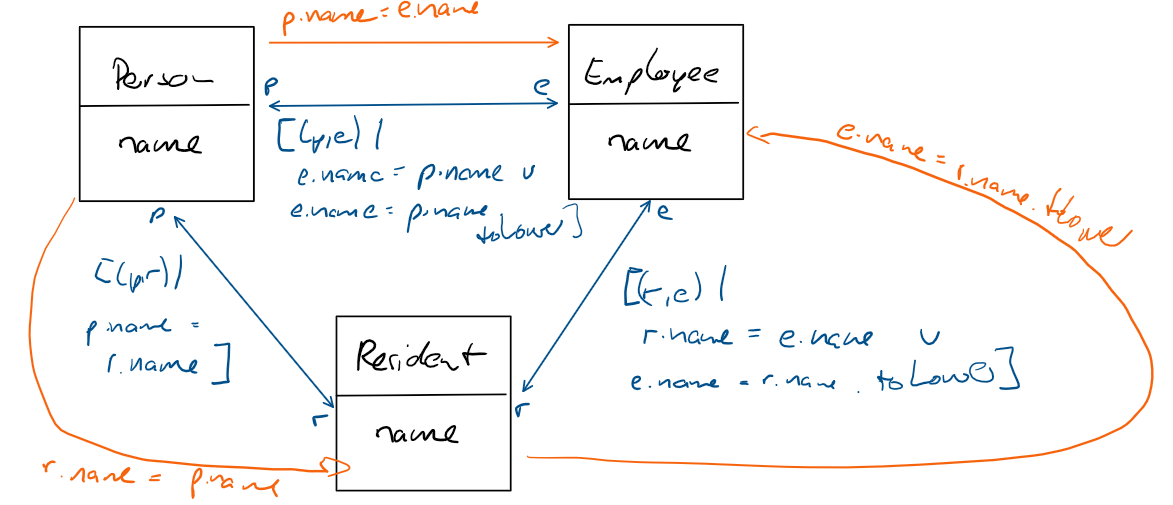
\includegraphics[width=0.9\textwidth]{figures/correctness/orchestration/confluence.png}
    \caption[Confluence of transformations counterexample]{Consistency relations and transformations representing a counterexample for the practicality of confluence in transformation networks.}
    \label{fig:orchestration:confluence}
\end{figure}

\mnote{Confluence definition}
Confluence is an even stronger requirement than the existence of an optimal orchestration.
In literature~\cite{stevens2020BidirectionalTransformationLarge-SoSym}, confluence in a transformation network is described as the property that for given models and changes a consistent orchestration exists, and that two consistent orchestrations for the same input always yield the same models.
Thus, executing transformations in any order such that the result is consistent will deliver the same result.
It is, however, easy to see that this is an impractical requirement.

\mnote{Counterexample for confluence}
In the example depicted in \autoref{fig:orchestration:confluence}, derived from the running example, three consistency relations expect for each person, employee, and resident the two corresponding others to exist.
They need to have the same $\mathvariable{name}$ or, in case of the relations between persons and employees as well as between residents and employees, the employee may have the same $\mathvariable{name}$ in lowercase.
The consistency preservation rule between persons and employees ensures that an employee with the same $\mathvariable{name}$ exists, whereas the one between residents and employees ensures that an employee with the $\mathvariable{name}$ in lowercase exists.
Whenever a person is added, two consistent orchestrations can be distinguished.
First, the transformation between persons and employees can be executed, either followed or preceded by the one between persons and residents. Then, all elements have the same $\mathvariable{name}$.
The models are also consistent to the relation between residents and employees, because the relation allows the names to be equal.
Alternatively, the transformation between persons and residents can be executed, followed by the one between residents and employees.
Then the employee has the $\mathvariable{name}$ in lowercase, but still this is consistent to the relation between persons and employees.

\mnote{Impracticality of confluence}
Apart from that artificial example, such a situation can always occur if transformations have different options for elements to be consistent.
If the overlap of consistent elements between all transformations does not contain a single element, the result may be any of the elements in the overlap.
And the result may depend on which transformation made the first selection that fell into the overlap.
This behavior is actually desired, thus preventing it by requiring confluence is not practical.
Finally, \textcite[p.~14]{stevens2020BidirectionalTransformationLarge-SoSym} also states that a network will only be confluent under very specific circumstances.

% Another intuitive notion of confluence would require that information flows together in a compatible way, i.e., the execution of a transformation does not violate consistency to other adjacent transformations.
% Formally this can be described as: A network is confluent when in every cycle of transformations t1,...tn the execution t1...ti-1 and tn,...,ti for any i leads to the same changes in the network.
% This means it does not matter in which order two transformations propagating information to the same model are executed.
% This, in consequence, means that the execution of a transformation cycles always yields models that are consistent to all transformations. Although two transformations affected the same model, consistency to the earlier executed one is not destroyed again.
% Finally, this reduces to the situation that executing each transformation once restores consistency to all transformations, which is, as we have seen, impractical.


